\begin{figure}[!htb]
    \centering
    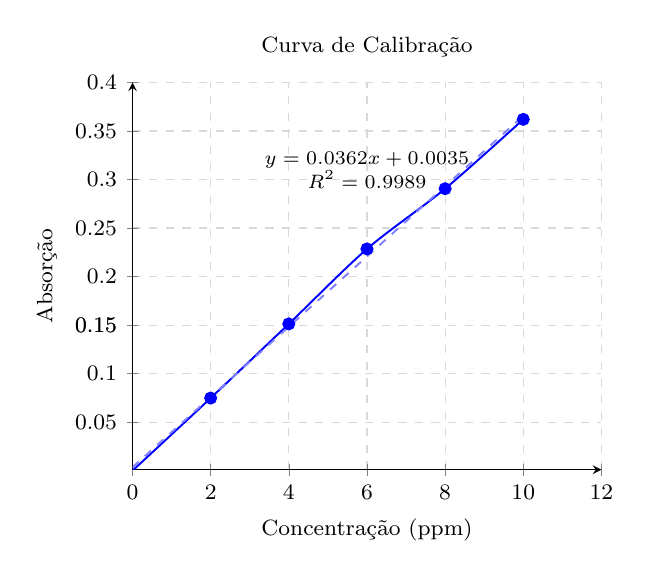
\begin{tikzpicture}[font=\footnotesize]
        \begin{axis}[
            title={Curva de Calibração},
            xlabel={Concentração (ppm)},
            ylabel={Absorção},
            xmin=0.001, xmax=12,
            ymin=0.001, ymax=0.4,
            ytick={0.05, 0.1, 0.15, 0.15, 0.2, 0.25, 0.30, 0.35, 0.40},
            yticklabel style={/pgf/number format/fixed},
            height=6.5cm,
            grid=major,
            grid style={dashed,gray!30},
            axis lines=left,
            legend pos=south east
        ]

        % Dados da tabela com linha suave entre pontos
        \addplot[
            mark=*,
            mark options={scale=1, fill=blue},
            color=blue,
            smooth,
            line width=0.7pt
        ] coordinates {
            (0, 0)
            (2, 0.07481)
            (4, 0.15123)
            (6, 0.22843)
            (8, 0.2905)
            (10, 0.36194)
        };

        % Linha de tendência (regressão linear)
        \addplot[
            domain=0:10,
            samples=100,
            color=blue!50,
            dashed,
            line width=0.7pt
        ]{0.0362*x + 0.0035};

        % Exibir a equação da linha de tendência e o R²
        \node at (axis cs:6,0.32) {\scriptsize $y = 0.0362x + 0.0035$};
        \node at (axis cs:6,0.30) {\scriptsize $R^2 = 0.9989$};

        \end{axis}
    \end{tikzpicture}
    \caption{Curva de calibração - Absorção Atómica.}
    \label{fig:curva-calibracao-aas}
\end{figure}